\documentclass[11pt,a4paper]{scrartcl}
\usepackage[czech]{babel}
\usepackage[utf8]{inputenc}
\usepackage{graphicx}
\usepackage{float}
\usepackage{gensymb}
\graphicspath{{./img/}}

\begin{document}
	\title{Semestrální práce z předmětu KIV/IR}
	\subtitle{Indexer}
	\author{Zdeněk Valeš}
	\date{26.5. 2020}
	\maketitle
	\newpage
	
	\section{Zadání}
	V jazyce Java vytvořte indexer, který bude schopný indexovat zadané dokumenty a následně nad nimi provádět vyhledávání. K realizaci práce použijte připravená rozhraní.
	
	\section{Analýza}
	Aplikace se skládá ze dvou částí. První část tvoří jádro, které indexuje dokumenty a vyhledává na základě dotazu, druhou část tvoří jednoduché grafické rozhraní pro práci s indexerem. Jádro aplikace se skládá z textového preprocesoru, indexu a vyhledávače.
	
	\subsection{Preprocessing}
	
	V průběhu pre-processingu textu dojde k jeho rozdělení na tokeny, vyřazení stop-slov a konečně k převodu do základní formy. Před rozdělením na tokeny jsou všechna písmena v textu převedena na malá a text je zbaven diakritiky. Součástí tokenizace je také odstranění kontrakcí v anglickém textu, respektive jejich převedení na celá slova. Regulární výrazy použité k detekci kontrakcí na svém GitHubu\footnote{https://gist.github.com/pauli31/3dce15096d87d8f32015ae519b32d418} publikoval uživatel pauli31. 
	
	Stop-slova jsou slova, jež typicky patří k nejběžnějším v jazyce, ale samotnému textu nedávají přílišný význam a jejich indexace je tedy zbytečná. Seznam stop-slov je pro každý jazyk jiný a neexistuje jeden univerzální. Protože jsem v průběhu cvičení stahoval anglický text, pre-processor primárně pracuje s anglickými stop- slovy\footnote{https://gist.github.com/sebleier/554280}. Aby bylo možné provést TREC evaluaci, je k dispozici také soubor s českými stop slovy. Algoritmus odstranění stop-slov spočívá v iterování přes text rozdělený na tokeny a v případě, že daný token odpovídá některému ze stop-slov, je z výsledného seznamu tokenů odstraněn.
	
	Stop-slova jsou uložena v 'nezákladní' formě (nejsou tedy zpracována stemmerem, nebo lemmatizérem) a proto se jejich vyhledání a odstranění z textu provádí ještě před jeho převedením na základní tvar.
	
	Token lze na základní tvar převést stematizací, nebo lemmatizací. Lemmatizace je o něco složitější a i když vrací gramaticky správný základní tvar (stemmer vrací kmen), není tento potřeba a proto jsem se rozhodl použít stemmer, místo lemmatizéru.
	
	\subsection{Index}
	Datová struktura pro ukládání zpracovaných dokumentů se nazývá index. Nejjednodušší formou indexu je tzv. incidenční matice o rozměrech $|D|\times|T|$, kde $D$ je množina uložených dokumentů a $T$ množina termů. V incidenční matici je pak každé dvojici dokument-term přiřazena hodnota 1 nebo 0, pokud se daný term v dokumentu nachází nebo ne. 
	 
	Tento způsob ukládání je značně neekonomický, protože většina hodnot v matici je 0 a ukládat gigabyty nul není žádoucí. Řešením je tzv. invertovaný index, což je struktura udržující seznam termů a pro každý term, seznam dokumentů, ve kterých se daný term vyskytuje -- tzv. postings list. Výhodou invertovaného indexu oproti incidenční matici je mimo jiné také možnost uložit počet výskytů termu v dokumentu, čehož jsem v práci využil při počítání TF-IDF vah.
	
	\subsubsection{Dokument}
	Kromě výskytů termů v dokumentu jsou také uložena jeho metadata. Základními metadaty, které vycházejí s poskytnutého rozhraní, jsou ID, text, titulek a datum. Protože jsem pracoval s komentáři ze stránky Reddit.com\footnote{https://old.reddit.com/r/politics/}, ve kterých jeden dokument představoval jeden komentář k příspěvku, přidal jsem k metadatům i skóre (suma souhlasných a nesouhlasných reakcí) a přezdívku autora komentáře. Rozhraní reprezentující metadata dokumentu je zobrazeno na obrázku \ref{fig:document-uml}.
	
	\begin{figure}[h]
		\centering
		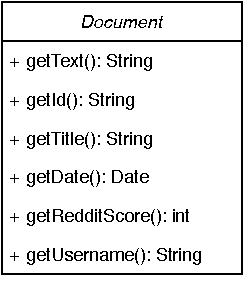
\includegraphics[width=0.3\linewidth]{document-uml}
		\caption{UML diagram rohzraní reprezentující dokument}
		\label{fig:document-uml}
	\end{figure}
	
	\subsubsection{TF-IDF váhy}
	Na dokument je, v rámci, indexu nahlíženo jako na množinu výskytů termů a konkrétní pozice termu v dokumentu není zohledněna. Tento přístup se nazývá \textit{bag of words model} a je založen na předpokladu, že dva dokumenty reprezentované podobnými množinami termů si budou také podobné.
	
	Jedním z klíčových ukazatelů podobnosti je počet výskytů TF$_{t,d}$, termu $t$ v dokumentu $d$. Ukazatel TF nicméně nezohledňuje důležitost termů a na všechny nahlíží jako na stejně rovné. Řešením je přidání váhy \textit{inverse document frequency}, definované jako IDF$_t=$log$\frac{N}{df_t}$. Tato přiřazuje vzácnějším termům vyšší váhu a naopak běžným termům vyskytujícím se ve velkém množství dokumentů váhu nižší. Výsledná TF-IDF váha termu $t$ v dokumentu $d$ je definovaná jako tf-idf$_{t,d}=$tf$_{t,d}\times$idf$_t$.  
	
	Pro zefektivnění vyhledávání jsou v indexu také uložené předpočítané IDF váhy termů, TF-IDF váhy termů v dokumentech a normy TF-IDF vektorů pro jednotlivé dokumenty. Původní verze programu tyto počítala během vyhledávání, což vedlo na velmi dlouhou dobu zpracování dotazu při TREC vyhodnocení (jednotky až desítky minut).
	
	\subsection{Vyhledávání v indexu}
	
	Vyhledávání v indexu pracuje ve dvou režimech: boolean retrieval a ranked retrieval. Boolean retrieval pracuje s booleovskými dotazy a vrací dokumenty, které přesně odpovídají dotazu. Oproti tomu ranked retrieval pracuje s výše zmíněnými TF-IDF vahamy, na základě kterých počítá podobnost dotazu s dokumentem a vrací dokumenty s nejvyšší podobností.
	
	\subsubsection{Boolean retrieval}

	Metoda vyhledávání pomocí booleovských dotazu je založena na vytvoření stromu dotazu, získání postings seznamů pro jeho listy a následného vypočtení průniku seznamů, podle booleovského operátoru, který je rodičem uzlů. Takto se postupuje od listů stromu až ke kořeni, kde je obsažen finální výsledek v podobě množiny dokumentů odpovídající dotazu.
	
	Aby bylo možné efektivně počítat průniky postings seznamů, je nutné aby tyto měly stejné řazení. Typicky se používá řazení podle ID dokumentu, nicméně ID dokumentu je v tomto případě řetězec, proto jsem seznamy seřadil podle zahashovaného ID.
	
	\subsubsection{Ranked retrieval}
	Vyhledávání pomocí podobnosti je založena na interpretaci dotazu jako dokumentu a následném výpočtu podobnosti s ostatními dokumenty. Dotaz je tedy, stejně jako dokumenty, převeden na vektor TF-IDF vah a podobnost mezi ním a dokumentem $d$ je vyjádřena jako kosinus úhlu, který mezi sebou tyto vektory svírají. Tato metoda výpočtu podobnosti se nazývá kosinová podobnost. Funkce kosinus je zvolena, protože pro totožné vektory (svírající úhel 0\degree) vrací 1 a pro naprosto odlišné (úhel 90\degree) vrací 0.
	
	Pro vektory $\vec{q}$ a $\vec{d}$ je kosinus úhlu $\alpha$, který mezi sebou svírají, definováno jako:
	
	\begin{equation}
		score_1(\vec{q}, \vec{d}) = cos \alpha = \frac{\vec{q} \cdot \vec{d}}{|\vec{q}| \cdot |\vec{d}|}
	\end{equation}
	
	Možnou optimalizací tohoto výpočtu je použití tzv. relativní kosinové podobnosti. Vektor dotazu $\vec{q}$ je nahrazen vektorem $\vec{Q}$, který se skládá pouze z hodnot 0 a 1 (1 pro každou ne-nulovou složku $\vec{q}$). Tím se skalární součin ve jmenovateli zjednoduší na součet (pro ne-nulové položky $\vec{Q}$) a celý vzoreček má tvar:
	
	\begin{equation}
		score_2(\vec{Q},\vec{d}) = \frac{\vec{Q} \cdot \vec{d}}{|\vec{d}|}
	\end{equation}
	
	Takto získaná hodnota sice již neudává kosinus úhlu mezi vektory, nicméně platí, že:
	
	\begin{equation}
		score_2(\vec{Q}, \vec{d_1}) \ge score_2(\vec{Q}, \vec{d_2}) \Leftrightarrow score_1(\vec{q}, \vec{d_1}) \ge score_1(\vec{q}, \vec{d_2})
	\end{equation}
	
	a proto lze tento zjednodušený vztah použít k výpočtu podobnosti dotazu a dokumentu.
	
	Při používání této metody typicky nechceme vrátit skóre každého dokumentu, ale jen $k$ nejrelevantnějších dokumentů. Protože $k$ je typicky výrazně menší než celkový počet dokumentů, není nutné provádět řazení nad všemi výsledky, ale stačí např. prvních 10. K tomu je použita halda do které jsou v průběhu výpočtu ukládány skóre jednotlivých dokumentů a po ukončení výpočtu je vybráno $k$ nejvyšších.
	
	\section{Popis implementace}
	Indexer byl implementován jako desktopová aplikace v jazyce Java, skládající se z jádra a grafického uživatelského rozhraní. Jádro aplikace je rozděleno mezi balíky \verb|core|, \verb|data| a \verb|preprocess|. K implementaci byla využita rozhraní ze zadání. 
	
	\subsection{Preprocessing}
	Logika předzpracování textu je obsažena ve třídě \verb|Preprocessor|. Tato třída tokenizuje a stemuje text pomocí dodaných tříd implementující rozhraní \verb|Tokenizer| a \verb|Stemmer|, tak jak je znázorněno na obrázku \ref{fig:preproc-uml}. Tím je zajištěna pohodlná rozšiřitelnost předzpracování.
	
	\begin{figure}[!h]
		\centering
		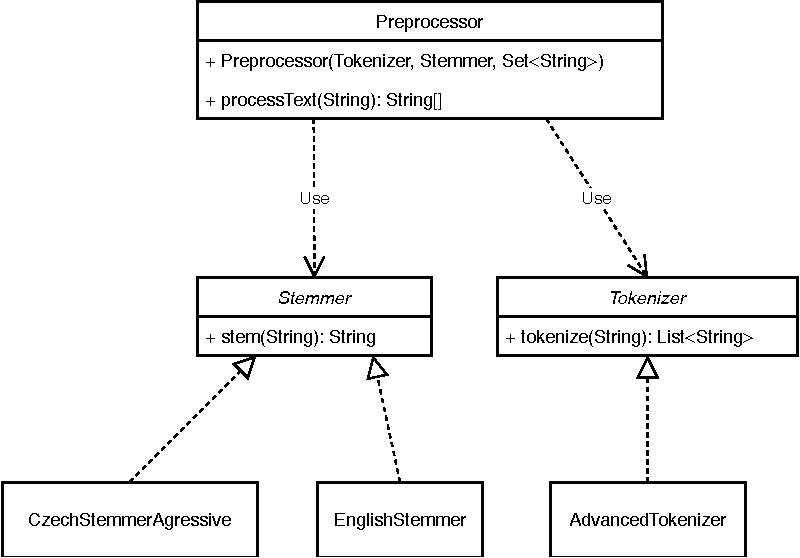
\includegraphics[height=8cm]{preproc-uml}
		\caption{Třídy zajišťující předzpracování textu}
		\label{fig:preproc-uml}
	\end{figure}

	Tokenizaci textu zajišťuje třída \verb|AdvancedTokenizer|, která vychází převázně z prací na cvičeních. Tokenizace textu je řešena následujícími regulárními výrazy:
	
	\begin{itemize}
		\item \verb|(http[s]?://[\\p{L}\d:/.?=\&+*-\_]+)| - detekce HTTP odkazů
		\item \verb|(\\p{L}[\\p{L}\d:/?=\&+*'-]+)| - detekce slov obsahující písmena, čísla a znaky
		\item \verb|(\d[\d*x.]+)| - detekce čísel a číselných výrazů
		\item \verb|<.*?>)| - detekce HTML tagů
		\item \verb|([\p{Punct}])| - detekce interpunkce
	\end{itemize}
	
	Tyto jsou spojeny operátorem $|$ do jednoho regulárního výrazu, kterým je text tokenizován.
	
	Stemování českého textu zajišťuje třída \verb|CzechStemmerAgressive| vytvořená během cvičení. Stematizátor anglického textu \verb|EnglishStemmer|, jež implementuje Porterův algoritmus, byl převzat z GitHub\footnote{https://github.com/stanfordnlp/CoreNLP/blob/master/src/edu/stanford/nlp/process/Stemmer.java} repozitáře CoreNLP.
	
	
	\subsection{Indexování}
	
	Třídy použité k indexování dokumentů jsou znázorněny na diagramu \ref{fig:index-uml}, zeleně označené jsou třídy dodané se zadáním. Samotná data jsou držena ve třídě \verb|InvertedIndex|, která reprezentuje invertovaný index. Kromě indexovaných dokumentů jsou zde uloženy také ID všech indexovaných dokumentů, předpočítané IDF hodnoty termů a normy TF-IDF vektorů dokumentů. 	Většina dat je ukládána do hashovacích map z důvodu snadného čtení.  
	
	\begin{figure}[!h]
		\centering
		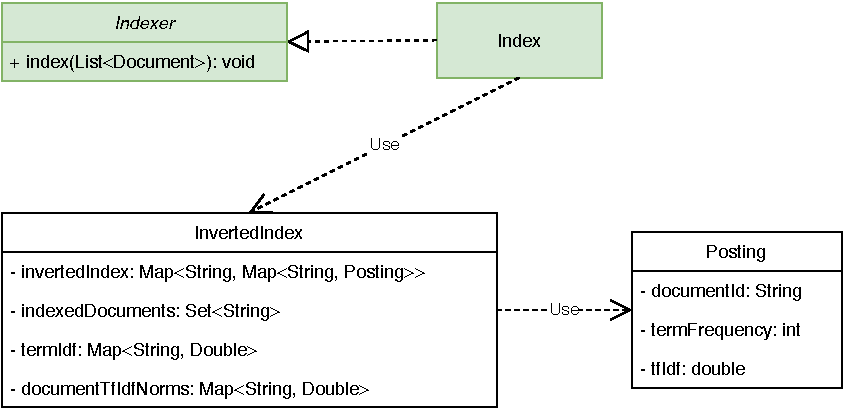
\includegraphics[height=6cm]{index-uml}
		\caption{Třídy zajišťující indexování dokumentů}
		\label{fig:index-uml}
	\end{figure} 

	Ve třídě \verb|InvertedIndex| se také nachází metody pro přepočítání TF-IDF vah termů, jež by měly být volané po indexování (aby byl index konzistentní). Atribut \verb|invertedIndex| obsahuje vnořenou \verb|Map|, jež umožňuje v seznamu postings vyhledávat pomocí dokument ID a není tedy nutné procházet celý seznam. 
	
	Aplikace podporuje ukládání indexu do soboru. V takovém případě je instance \verb|InvertedIndex| serializována a uložena do zadaného souboru. Nevýhodou tohoto přístupu je závislost na implementaci a pokud ve třídě \verb|InvertedIndex|  dojde ke změně, staré soubory s indexem již nejsou kompatibilní.
	
	Dokumenty do indexu lze také načíst ze souboru, nicméně protože je tato funkcionalita určena pro data, která jsem sebral crawlováním stránky Reddit během cvičení, je popdporován pouze specifický formát JSON. Soubor musí obsahovat pole JSON objektů, jež mají atributy \verb|username|, \verb|timestamp|, \verb|score| a \verb|text|. Parsování JSON souborů je implementováno ve třídě \verb|RPolDocumentReader|.
	
	\subsection{Vyhledávání}
	
	Vyhledávání nad indexem je prováděno skrze dodané rozhraní \verb|Searcher|. Diagram \ref{fig:search-uml} popisuje strukturu tříd, zajišťujících rozparsování dotazu a následné vyhledání relevantních dokumentů.
	
	\begin{figure}[!h]
		\centering
		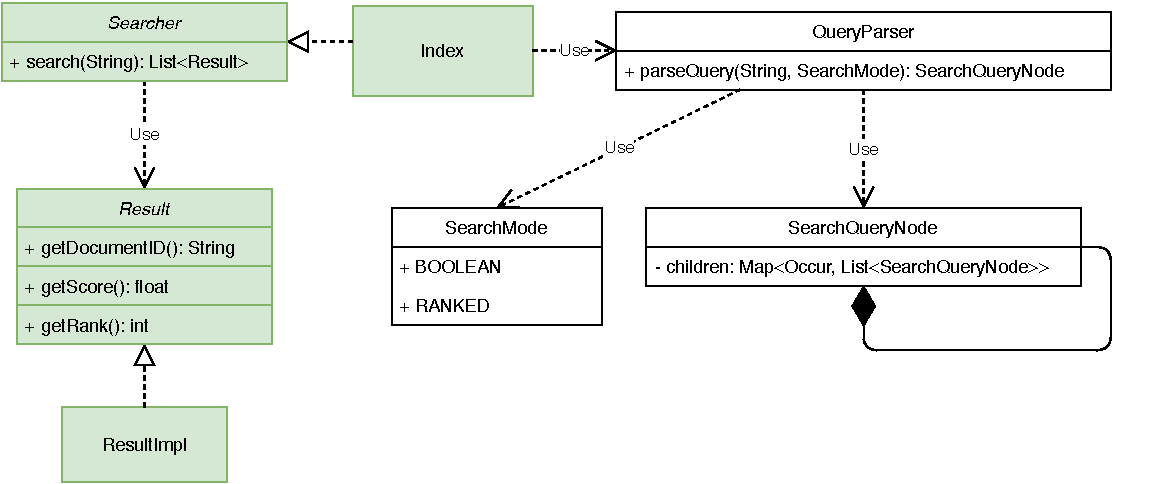
\includegraphics[width=\linewidth]{search-uml}
		\caption{Třídy zajišťující vyhledání dokumentů v indexu}
		\label{fig:search-uml}
	\end{figure} 
	
	Aplikace podporuje dva režimy vyhledávání (boolean a ranked). Tyto jsou reprezentovány enumem \verb|SearchMode|, jež slouží k výběru parsovací metody a také k výběru vyhledání dokumentů. Zpracování dotazů (pro oba režimy) je implementováno ve třídě \verb|QueryParser|. Vnitřně je k parsování použita knihovna Lucene. Třída \verb|SearchQueryNode| je rekurzivním objektem použitým k reprezentaci booleovských dotazů stromem. 
	
	\begin{figure}[!h]
		\centering
		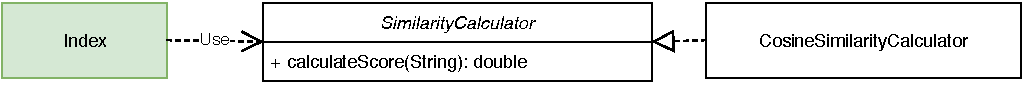
\includegraphics[width=\linewidth]{cosine-uml}
		\caption{Třídy pro počítání ranked retrieval}
		\label{fig:cosine-uml}
	\end{figure} 
	
	V případě vyhledávacího režimu ranked je k výpočtu skóre použita metoda kosinové podobnosti. Diagram \ref{fig:cosine-uml} obsahuje rozhraní \verb|SimilarityCalculator|, protože původní záminka byla implementovat více modelů podobnosti. Nicméně z časových důvodů bylo od tohoto upuštěno a jedinou implementací je tedy třída \verb|ConsineSimilarityCalculator|, jež využívá model kosinové podobnosti. 
	
	\subsection{Uživatelské rozhraní a jeho ovládání}
	
	Uživatelské rozhraní bylo implementováno pomocí frameworku Java Swing. Teto jsem si vybral kvůli jeho jednoduchosti a znalosti z předchozích prací. Celé rozhraní, které je zobrazeno na obrázku \ref{fig:gui-example}, je rozděleno do dvou hlavních částí. Těmi jsou vyhledávací panel (vlevo) a panel pro ovládání indexu (vpravo).
	
	\begin{figure}[!h]
		\centering
		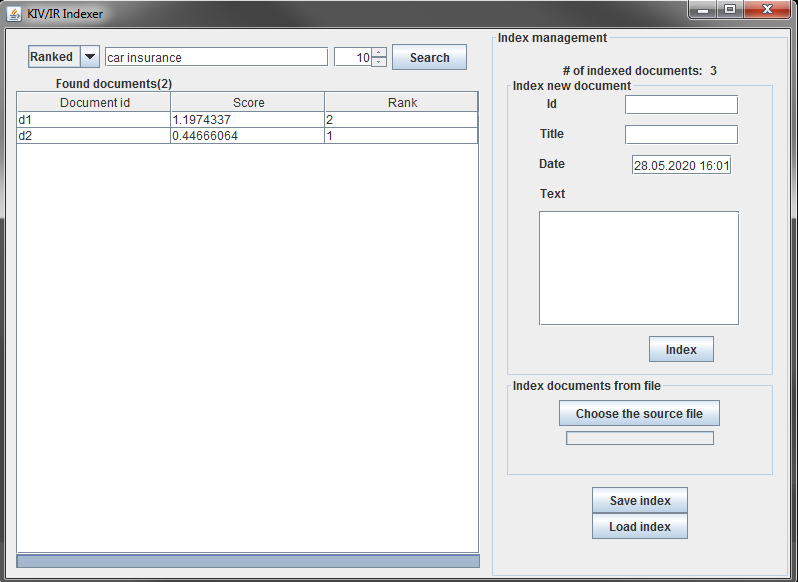
\includegraphics[width=0.9\linewidth]{gui-ranked}
		\caption{Ukázka grafického rozhraní aplikace}
		\label{fig:gui-example}
	\end{figure}

	\subsubsection{Ovládání indexu}
	
	Panel pro ovládání indexu obsahuje kontrolní prvky pro indexování jednotlivých dokumentů, indexování dokumentů ze souboru a pro uložení indexu do souboru a jeho případné načtení.
	
	Pro indexování jednotlivých dokumentů je potřeba vyplnit pole Id, Title a Text (všechna jsou povinná) a následně kliknout na tlačítko \textit{Index}. V případě úspěchu se počet indexovaných dokumentů v horní části panelu zvýší o jedna, v opačném případě je zobrazena chybová hláška.
	
	Indexování dokumentů ze souboru je určeno pro načítání dat, které jsem získal během prvních cvičeních. Výběr souboru a jeho následné rozparsování a oindexování lze provést kliknutím na tlačítko \textit{Choose the source file}. Protože indexování velkého počtu dokumentů může trvat delší čas, je pod tlačítkem umístěna komponenta pro sledování průběhu indexování. 
	
	Index je možné uložit do souboru kliknutím na tlačítko \textit{Save idnex}. Jeho opětovné nahrání je možné kliknutím na tlačítko \textit{Load index}.

	\subsubsection{Vyhledávání}

	Vyhledávací panel se skládá z vyhledávacího formuláře a tabulky pro zobrazení výsledků. Jak již bylo řečeno, vyhledávač umí pracovat ve dvou režimech - ranked a boolean retrieval. Režim vyhledávání lze vybrat komponentou v levé straně vyhledávacího formuláře. Omezení počtu výsledků lze nastavit číselným výběrem. Vyhledávání lze spustit kliknutím na tlačítko \textit{Search}. Podobně jako u indexování, i tato akce může trvat nějakou dobu a proto je ve spodní části vyhledávacího panelu (pod tabulkou s výsledky) umístěn progress bar, kterýám lze sledovat postup vyhledávání.   
	
	Příklady zobrazení výsledků v tabulce pro jednotlivé režimy jsou na obrázcích \ref{fig:ranked} a \ref{fig:boolean}. V případě boolean retrieval je hodnota skóre 1, protože dokument buď přesně odpovídá dotazu (1), nebo neodpovídá a není tedy uveden ve výsledcích. Nad tabulkou je umístěn také indikátor počtu vrácených dokumentů.

	\begin{figure}[h]
		\centering
		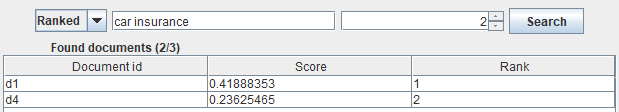
\includegraphics[width=\linewidth]{gui-ranked-res}
		\caption{Výsledky ranked retrieval}
		\label{fig:ranked}
	\end{figure}

	\begin{figure}[h]
		\centering
		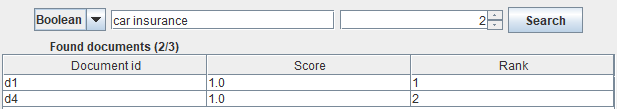
\includegraphics[width=\linewidth]{gui-boolean-res}
		\caption{Výsledky boolean retrieval}
		\label{fig:boolean}
	\end{figure}
	
	\section{Závěr}
	
	Práce byla implementována
	
\end{document}
